\section{Building coherent signal subnetworks}
\label{sec:ch9:ssn_coherent}

In Section \ref{sec:ch9:ssn_incoherent}, we learned how to estimate a signal subnetwork from a set of networks which are in one of $K$ classes. We then covered how to use this estimated signal subnetwork to train a classifier which uses the signal edges to make predictions of the class for new networks. We learned how to use cross validation to tune the number of edges in the estimated signal subnetwork, so that we could identify the number of edges in the signal subnetwork which maximized the downstream classification accuracy for new networks. 

However, we had a slight problem: Even when we tuned the network using cross validation, we still tended to miss the edge between the sight areas (SI) and the language areas (L), as shown in Figure \ref{fig:ch9:ssn:ssn_inco_edgeimp}(C). This edge was truly a signal edge, even though the signal that it carries (a difference in probabilities between the astronauts and the earthlings) is less than some of the other signal edges, which is shown in Figure \ref{fig:ch5:ssg_pmtxs}(C). At an extremely high level, even though this edge does not convey much signal by itself, it conveys signal that is helpful (in the grand scheme of things) for our subsequent prediction. 

At a more technical level, a classifier which leverages all signal edges in its predictions achieves a higher \textit{Bayes accuracy} \cite{Vogelstein2013Jul,Fukunaga1990Oct}. The Bayes accuracy is the highest possible classification accuracy that can be achieved by a classifier which knows the true underlying data generating distribution. Without going into too much technical detail, the idea is that achieving optimal performance (via a \textit{Bayes optimal} classifier) requires a classifier which leverages information from all signal edges, as ignoring signal edges will inherently ``discard'' useful information about the underlying data generating distribution.

The problem here is that the preceding signal subnetwork estimator was an incoherent estimator. An \textit{incoherent signal subnetwork estimator} is an estsimator for a signal subnetwork which does not take into consideration the structure of a network when determining the edges to include in the signal subnetwork. This is obvious from our preceding section: the signal subnetwork which is estimated looks *only* at the edges which have the highest edge importance (quantified by the edges with the lowest Fisher's exact test $p$-value) when deciding which edges to include, or exclude, from the signal subnetwork estimator. This is an incoherent estimator because it disregards the structure of the network; that is, a collection of not just edges, but also, nodes which convey information. On the other hand, we will now learn about a coherent signal subnetwork estimator. A \textit{coherent signal subnetwork estimator} is an estimator of a signal subnetwork which leverages the structure of the network, by using at least two elements of its structure: nodes, edges, or other network attributes.

To begin this section, we will reconstruct our data examples that we created previously. This time, we will obtain $200$ training and testing samples explicitly:

\begin{lstlisting}
import numpy as np
from graspologic.simulations import sample_edges

# generate probability matrices
n = 5  # the number of nodes
P_earthling = 0.3*np.ones((n, n))
signal_subnetwork = np.zeros((n, n), dtype=bool)
signal_subnetwork[1:n, 0] = True
signal_subnetwork[0, 1:n] = True
P_astronaut = np.copy(P_earthling)
P_astronaut[signal_subnetwork] = np.tile(np.linspace(0.4, 0.9, num=4), 2)

# sample the classes of each sample
M = 200  # the number of training and testing samples
pi_astronaut = 0.45
pi_earthling = 0.55
ytrain = np.random.choice(2, p=[pi_earthling, pi_astronaut], size=M)
ytest = np.random.choice(2, p=[pi_earthling, pi_astronaut], size=M)

# sample network realizations given the class of each sample
Ps = [P_earthling, P_astronaut]
Atrain = np.stack([sample_edges(Ps[y]) for y in ytrain], axis=2)
Atest = np.stack([sample_edges(Ps[y]) for y in ytest], axis=2)
\end{lstlisting}

Let's consider what is happening using coin flips. The edge $(SI, L)$ could be represented by a coin which lands on heads with probability $0.4$ for astronauts, but $0.3$ for earthlings. In a given set of networks of earthlings and astronauts, we could think about the existence or not existence of this particular edge in our heads or tails framework. There is a chance that the rate we see heads for astronauts is the same, or even less, than the rate we see heads for earthlings. 

Now, let's imagine another experiment for a non-signal edge, such as $(L, H/E)$ between the language node and the hearing/emotion node. In this case, this edge is a non-signal edge, which could be represented by a coin which lands on heads with probability $0.3$ for both astronauts and earthlings alike. In a given set of networks of earthlings and astronauts, it is possible that we still see more heads in one group or the other, and this turns out to be estimated to be a signal edge by our procedure for estimating signal subnetworks using the approach we described in Section \ref{sec:ch9:ssn_incoherent}. 

When we have a lot of non-signal edges, and only a small subset of signal edges, the chances of us running into this problem somewhere along the way grows. This is closely related to the multiple comparisons problem that we were first introduced to in Section \ref{sec:ch7:testing:twosample}, where we might see spuriously small $p$-values (and consequently, high edge importances) in non-signal edges simply due to random chance a fraction of the time. 



\subsection{Building a coherent signal subnetwork estimator}

To reduce this type of sample-specific noise, we can use more information about our networks: the nodes that the edges are between. What we will do is something like this: we compute the ranked significance matrix, *exactly* as we did before. However, when we pick the edges to include, or exclude, we first choose the $V$ nodes (the \textit{signal nodes}) which tend to have the highest ranked significances. We then identify the $K$ signal edges using only edges which have at least one node as a signal node. This approach produces a coherent signal subnetwork estimate because it uses both the nodes and the edges when deciding the signal subnetwork estimate, and therefore incorporates other useful elements of the network structure (the nodes) when determining the signal subnetwork estimator. 

At a high level, the procedure to build a coherent signal subnetwork estimator is described in Algorithm \ref{alg:ch9:ssn_coherent}.


\begin{algorithm}
\label{alg:ch9:ssn_coherent}
\caption{Building a coherent signal subnetwork estimator}
\KwData{A set of networks and class labels $\left(A^{(m)}, y_m\right)$, for $m = 1, \hdots, M$. \newline
$V$ the number of signal nodes. \newline
$K$ the number of signal edges.}
\KwResult{$(\mathcal S, \mathcal V)$ a set of signal edges and signal nodes in the network.}
\SetAlgoLined

Compute the ranked significance matrix $R$, which is an $n \times n$ matrix whose entries $r_{ij}$ are the ranked significance for edge $i$ and $j$.

Initialize $c = \max_{i,j}r_{ij}$, and let $w_c = 0$.

\While{$w_c < K$}{
    For each node $i$, let $w_{i, c} = \sum_{j = 1}^n \mathfrak 1\left\{r_{ij} \geq c\right\}$ to be the number of edges for node $i$ where the ranked significance is at least $c$.

    Rank the nodes according to which node has the number of signal edges exceeding the threshold $c$. Denote the $i^{th}$ largest node by $w_{(i),c}$. 

    Let $w_c = \sum_{i = 1}^V w_{(i), c}$ be the sum of the number of edges each of the top $V$-ranked nodes have at least at the threshold $c$. 

    Let $c = c - 1$.
}

Let $\mathcal V$ be the node set of the top $V$ nodes identified in the final iteration of the preceding while loop.

Let $\mathcal S$ be the top $K$ signal edges where at least one node for each edge is in the signal node set $\mathcal V$.

\Return{$(\mathcal S, \mathcal V)$.}
\end{algorithm}

Conceptually, this process entails finding an appropriate threshold, $c$, such that the top $V$ signal nodes have at least $K$ signal edges with a ranked significance at least $c$. Then, we simply identify the coherent signal subnetwork estimate as the top $K$ edges where at least one node is in the signal node set $\mathcal V$.

We can do this using \texttt{graspologic} using multiple constraints, as follows, where we compute both incoherent and coherent signal subnetwork estimates:

\begin{lstlisting}[style=python]
from graspologic.subgraph import SignalSubgraph
K = 8  # the number of signal edges
V = 1  # the number of signal nodes

# the incoherent signal subnetwork estimator
ssn_est_inco = SignalSubgraph()
ssn_est_inco.fit_transform(Atrain, labels=ytrain, constraints=K)

# the coherent signal subnetwork estimator
ssn_est_coherent = SignalSubgraph()
ssn_est_coherent.fit_transform(Atrain, labels=ytrain, constraints=[K, V])
\end{lstlisting}

We can build the signal subnetworks to visualize them, using the same code that we used previously:

\begin{lstlisting}[style=python]
ssn_coherent = np.zeros((n, n))
ssn_incoherent = np.zeros((n, n))

ssn_incoherent[ssn_est_inco.sigsub_] = 1
ssn_coherent[ssn_est_coherent.sigsub_] = 1
\end{lstlisting}

\begin{figure}
    \centering
    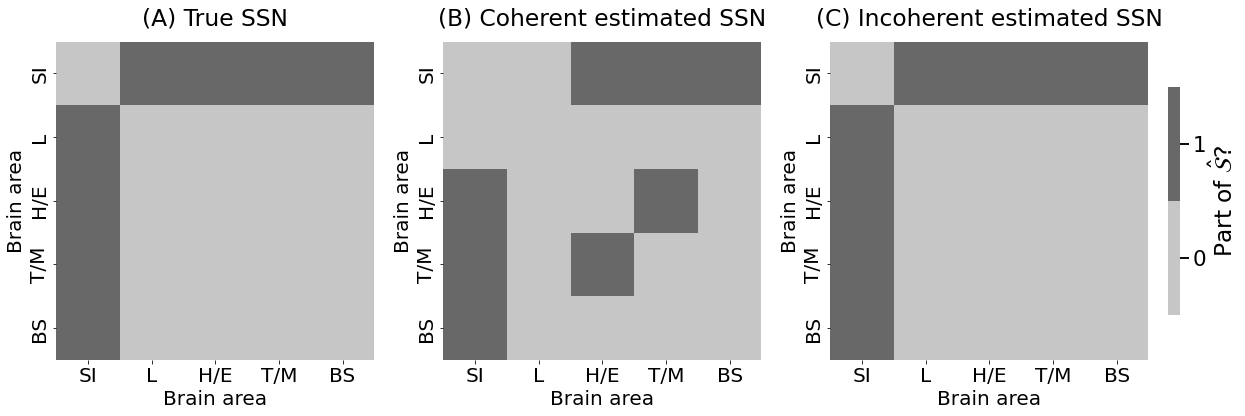
\includegraphics[width=\linewidth]{applications/ch9/Images/ssn_co.png}
    \caption[Comparing coherent and incoherent signal subnetwork estimates.]{\textbf{(A)} the true signal subnetwork, \textbf{(B)} the incoherent signal subnetwork estimate, \textbf{(C)} the coherent signal subnetwork estimate.}
    \label{fig:ch9:ssn:ssn_coh}
\end{figure}
A visualization of the true signal subnetwork, the incoherent signal subnetwork, and the coherent signal subnetwork is shown in Figure \ref{fig:ch9:ssn:ssn_coh}. Although the incoherent signal subnetwork estimate will sometimes have spurious edges which are non-signal edges included, the coherent signal subnetwork estimate will (with far higher probability) only include the signal edges for the signal node (the SI node). 

Now that we have our intuition built up, we can put this together for training and evaluating coherent signal subnetworks, using similar code to that which we used previously:

\begin{lstlisting}[style=python]
def train_and_eval_coherent_ssn(Atrain, ytrain, Atest, ytest, K, V):
    """
    A function which trains and tests an incoherent signal subnetwork
    classifier with K signal edges and V signal nodes.
    """
    ssn_est = SignalSubgraph()
    ssn_est.fit_transform(Atrain, labels=ytrain, constraints=[int(K), int(V)]);

    Dtrain = Atrain[ssn_est.sigsub_[0], ssn_est.sigsub_[1],:].T
    classifier = BernoulliNB()
    # fit the classifier using the vector of classes for each sample
    classifier.fit(Dtrain, ytrain)

    # compute testing data on the estimated signal subnetwork
    Dtest = Atest[ssn_est.sigsub_[0], ssn_est.sigsub_[1],:].T
    yhat_test = classifier.predict(Dtest)
    
    # classifier accuracy is the fraction of predictions that are correct
    return (np.mean(yhat_test == ytest), ssn_est, classifier)
\end{lstlisting}

\subsubsection{Parameter selection for coherent signal subnetworks}

We again turn to cross validation for parameter selection for coherent signal subnetworks. Whereas in Algorithm \ref{alg:ch9:ssn} we only addressed parameter selection for incoherent signal subnetworks, we can use the same intuition to develop a method to parameter select for coherent signal subnetworks. In this case, we can simply add an additional loop to our computation, where we also tune over the number of signal nodes to include in the estimate. Our procedure for training and testing with a classifier is exactly the same as it was before.

\begin{lstlisting}[style=python]
from sklearn.model_selection import KFold
import pandas as pd

kf = KFold(n_splits=20, random_state=None)
xv_res = []
for l, (train_index, test_index) in enumerate(kf.split(range(0, M))):
    A_train, A_test = Atrain[:,:,train_index], Atrain[:,:,test_index]
    y_train, y_test = ytrain[train_index], ytrain[test_index]
    nl = len(test_index)
    
    for k in np.arange(2, n*(n-1), step=2):
        for v in range(1, n+1):
            try:
                acc_kl = train_and_eval_coherent_ssn(A_train, y_train, A_test, y_test, k, v)[0]
                xv_res.append({"Fold": l, "k": k, "nl": nl, "v": v, "Accuracy": acc_kl})
            except:
                xv_res.append({"Fold": l, "k": k, "nl": nl, "v": v, "Accuracy": np.nan})
xv_data = pd.DataFrame(xv_res)

def weighted_avg(group):
    acc = group['Accuracy']
    nl = group['nl']
    return (acc * nl).sum() / nl.sum()

xv_acc = xv_data.groupby(["k", "v"]).apply(weighted_avg).reset_index(name='Accuracy')
# convert the pandas dataframe (long format) to a data matrix (wide format)
df_hm = xv_acc.pivot("k", "v", "Accuracy")
\end{lstlisting}

We made a slight augmentation to the code, including a \texttt{try}/\texttt{except} block. The reason for this is that $20$ signal edges is only possible with $5$ signal nodes, so for any number of signal nodes less than $5$, we will not be able to find a signal subnetwork with $20$ signal edges. The accuracies are plotted as a heatmap in Figure \ref{fig:ch9:ssn:ssn_inco_acc}(A). 

\begin{figure}
    \centering
    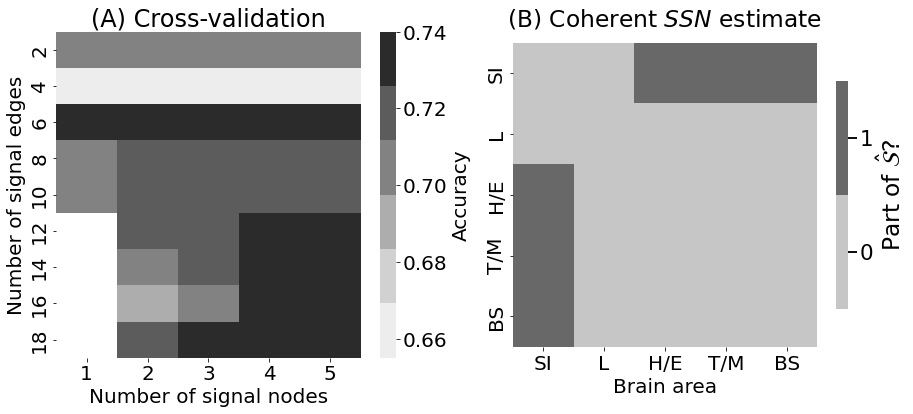
\includegraphics[width=0.8\linewidth]{applications/ch9/Images/ssn_inco_acc.png}
    \caption[Cross-validated accuracy heatmap for coherent $SSN$]{\textbf{(A)} the cross-validated accuracy as a heatmap for a coherent $SSN$, as a function of the number of signal nodes and edges, \textbf{(B)} the estimated signal subnetwork from the training data with the ``optimal'' number of signal nodes and signal edges.}
    \label{fig:ch9:ssn:ssn_inco_acc}
\end{figure}
While many combinations produce the same cross-validated accuracy, all-else-equal, it is typically best practice (to avoid overfitting) to choose the simplest model (in terms of the number of free parameters). In this case, the simplest model which attains the highest cross-validated accuracy is with $1$ signal node and $6$ signal edges. When we refit the model on the full training data, we get:

\begin{lstlisting}[style=python]
# the coherent signal subnetwork estimator, using the parameters from xv
ssn_est_coherent_xv = SignalSubgraph()
ssn_est_coherent_xv.fit_transform(Atrain, labels=ytrain, constraints=[1, 6])

ssn_coherent_xv = np.zeros((n, n))
ssn_coherent_xv[ssn_est_coherent_xv.sigsub_] = 1
\end{lstlisting}

or the signal subnetwork shown in Figure \ref{fig:ch9:ssn:ssn_inco_acc}(B). The testing accuracy on the held-out testing data can be computed as previously:

\begin{lstlisting}[style=python]
Dtrain_xv = Atrain[ssn_est_coherent_xv.sigsub_[0], ssn_est_coherent_xv.sigsub_[1],:].T
classifier_xv = BernoulliNB()
# fit the classifier using the vector of classes for each sample
classifier_xv.fit(Dtrain, ytrain)

# compute testing data on the estimated signal subnetwork
Dtest = Atest[ssn_est_coherent_xv.sigsub_[0], ssn_est_coherent_xv.sigsub_[1],:].T
yhat_test = classifier_xv.predict(Dtest)

accuracy = np.mean(yhat_test == ytest)
\end{lstlisting}